\centering
\begin{subfigure}[b]{0.3\textwidth}
    \centering
    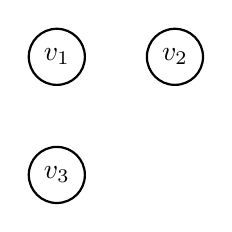
\begin{tikzpicture}[node distance={15mm}, thick, main/.style = {draw, circle}]
        \node[main] (1) {$v_1$};
        \node[main] (2) [right of=1] {$v_2$};
        \node[main] (3) [below of=1] {$v_3$};
    \end{tikzpicture}
    \caption{$G_{t_3}$}
    \label{f_ctdg_1}
\end{subfigure}
\begin{subfigure}[b]{0.3\textwidth}
    \centering
    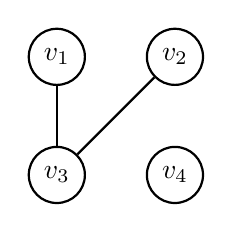
\begin{tikzpicture}[node distance={15mm}, thick, main/.style = {draw, circle}]
        \node[main] (1) {$v_1$};
        \node[main] (2) [right of=1] {$v_2$};
        \node[main] (3) [below of=1] {$v_3$};
        \node[main] (4) [below of=2] {$v_4$};
        \draw (1) -- (3);
        \draw (2) -- (3);
    \end{tikzpicture}
    \caption{$G_{t_6}$}
    \label{f_ctdg_2}
\end{subfigure}
\begin{subfigure}[b]{0.3\textwidth}
    \centering
    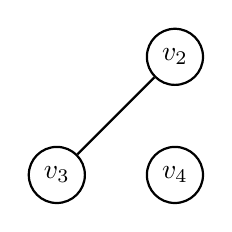
\begin{tikzpicture}[node distance={15mm}, thick, main/.style = {draw, circle}]
        \node[main] (3) {$v_3$};
        \node[main] (4) [right of=3] {$v_4$};
        \node[main] (2) [above of=4] {$v_2$};
        \draw (2) -- (3);
    \end{tikzpicture}
    \caption{$G_{t_8}$}
    \label{f_ctdg_3}
\end{subfigure}